\subsection{Sensing Subsystem}
\label{sec:sensing_subsystem}
The sensing subsystem is an infrared spectrometer that uses two photodiodes as detectors, a diffraction grating as a spectral separator, an array of LEDs to illuminate the target area, and optics to collect, collimate, and focus the beam. In order to determine the component positions and interaction, each component will have to be addressed.
\begin{figure}[H]
    \caption{Sensing subsystem block diagram}
    \centering
    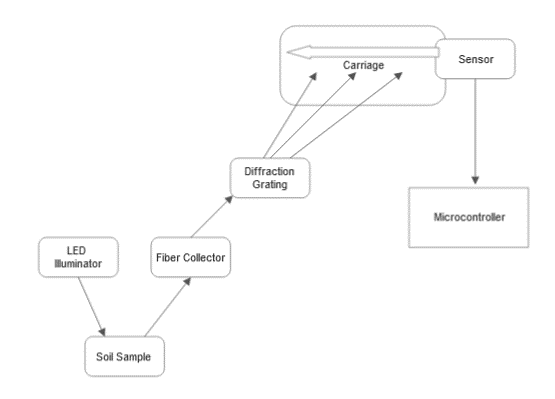
\includegraphics[width=0.75\textwidth]{images/OpticsBlockDiagram.png}
\end{figure}


\paragraph{Overview} Soil is a heterogeneous combination of organic and inorganic substances, and the balance of soil nutrients contributes directly to the quality of the garden environment. Each substance contributes to the total radiative emission of the soil, so by measuring the electromagnetic waves from a sample with unknown quantities and comparing it to output from a sample with known quantities, the nutrients can be estimated. Soil Carbon content, Moisture Content, Phosphorous, and pH can all be detected within the 400nm to 1700nm range.
The sensing subsystem is made up of three smaller composite systems. The collection group generates and guides an electromagnetic wave into the spectrometer housing. The scanning group separates that wave into many directions and then passes a sensor through the spatially separated beams. The circuit group converts the optical power into an electrical current, then into a voltage, then records that voltage for analysis. The Microcontroller system will then use that data for decision-making.

\subsubsection{Collection Group}

The collection group is made up of 4 parts: The tungsten-halogen lamp, the acrylic block, the fiber collimator, and the fiber cable. Its purpose is to direct light into the dirt, to cause it to emit electromagnetic waves, and to guide those waves into the spectrometer housing.

\paragraph{Tungsten Lamp} Tungsten is a material which emits a broad range of frequencies, covering the spectrum of interest and then some. This light bulb generates the optical power that will excite the soil sufficiently for spatially separated wavelengths to be detected. If the optical power is too weak, it can be boosted by confining the light around the soil using a reflector shield, or the number of bulbs can be increased.

\begin{figure}[H]
    \caption{Spectral Output of a Tungsten Lamp}
    \centering
    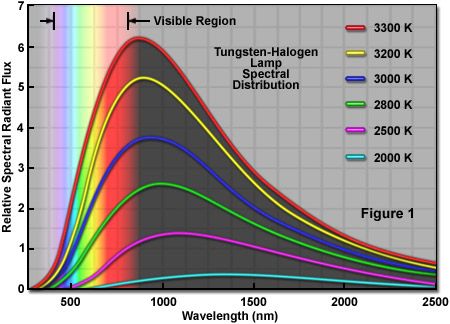
\includegraphics[width=0.75\textwidth]{images/TungstenLamp.jpg}
\end{figure}

\paragraph{Acrylic Block} The optical signal emitted by the soil will be weak, so it is essential that the spectrometer is influenced as much as possible by the content of the soil and as little as possible by the topology of the surface. A well-mixed, smoothly flattened, gently compressed soil sample provides the best conditions for constructing a spectrograph. If there are ridges or depressions along the sample, too much or too little optical signal will pass into the spectrometer, creating an apparent signal strength for wavelengths that is not representative of the soil emission. There are several ways to control these conditions. One is to require the user to retrieve a sample for each scan and deposit it into a spectrometer bay. Another is to require the user to flatten the soil with a spatula or other implement and position the scanner input near the soil. These reduce ease of use, which is a target for the project. Another issue is that the position of the signal input and the tungsten light source relative to the soil sample will have to be consistent to avoid signal error, for the same reasons as above. In (reference) study, this issue was resolved by building a transparent block with slots to hold the light source and the input beam. Their design is represented below, showing the block attached at the rear of a plow chisel for clearing soil while scanning. We will solve the problem of soil topology and light position the same way, by mounting the light source and input fiber in a block of some transparent material like acrylic. This has the added functionality of protecting the surface of the lens from dirt and water, which introduce a myriad of contaminants and deteriorate signal quality. The downside of using a cheap material is that it may introduce obstacles to spectroscopy through unwanted reflection and absorption.

\begin{figure}[H]
    \caption{Fiber Position in Soil Drill}
    \centering
    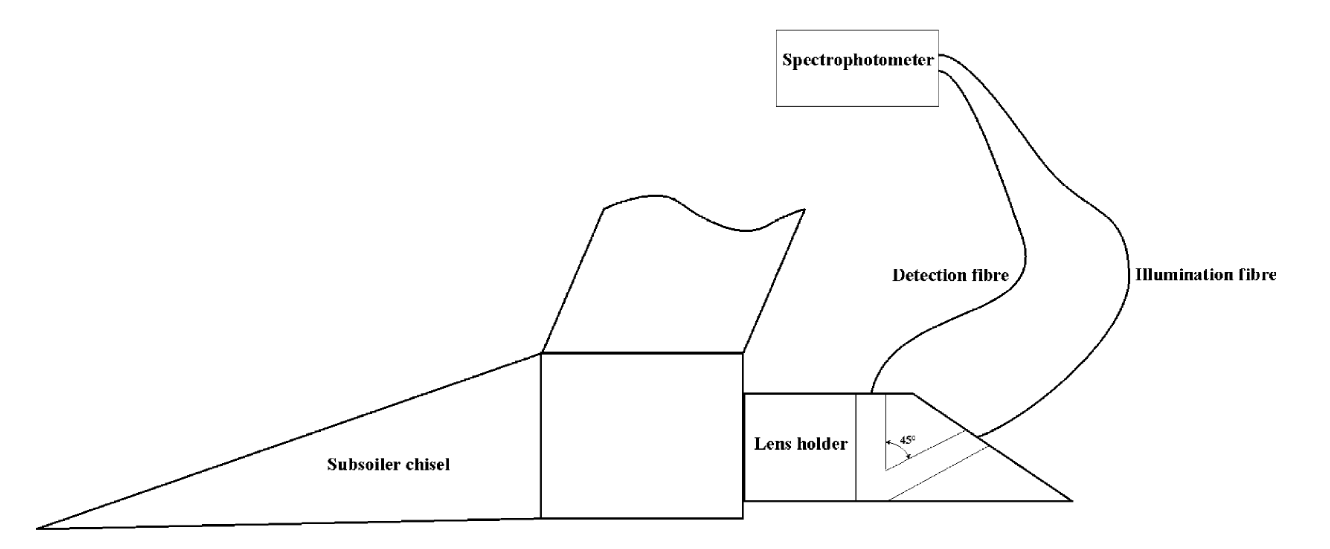
\includegraphics[width=0.75\textwidth]{images/Acrylic Block Fiber positioner.png}
\end{figure}

\paragraph{Fiber Optics} Fiber optic cables are a standard input for spectrometer devices since they allow nearly unlimited flexibility for the position and orientation of the target area relative to the device. The basic ray trace for a lens coupling light into a fiber is shown below. Fiber cores face some basic limitations when it comes to coupling. The maximum possible coupling efficiency can be achieved by pressing the optical surface of the fiber core up against a light source with equal random output in every direction (reference). If the fiber is moved some distance away from the source, less light will impede on the core-air interface. If the core diameter is increased, this will increase the light incident on the core. Light moving in random directions will also strike the fiber core at various angles, however, not all angles of incidence will couple into the fiber. Only rays within the numerical aperture of the fiber will be accepted. This is why installing large lenses at the end of the fiber does not increase the maximum possible amount of light that can be coupled. The maximum angle is determined by the fiber, rather than the collimator.

\begin{figure}[H]
    \caption{Coupling a diffuse light into a fiber}
    \centering
    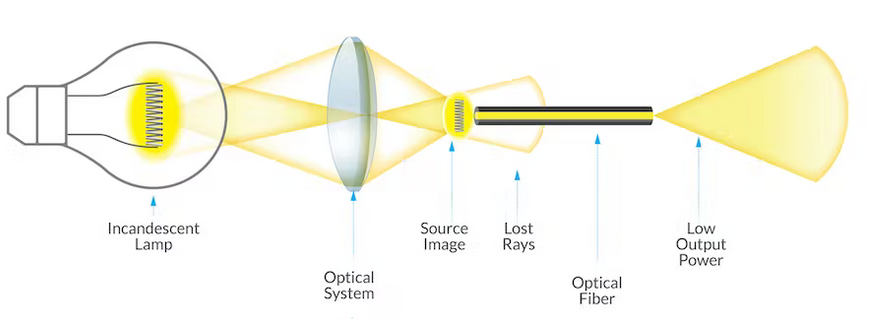
\includegraphics[width=0.75\textwidth]{images/CouplingDiffuseLighttoFiber.png}
\end{figure}

This project involves a large diffuse source, the illumined soil. The Fiber collimator will be attached to the fiber cable via their SMA connectors, then the collimator will be set in an acrylic block so that it rests 8.06mm above the soil. The block will also have a slot for the Light source to illuminate the soil at an angle, similar to the arrangement of the source and sensor in a computer mouse above a mousepad.
The signal will travel through the fiber and up into the spectrometer housing, where the other connector of the cable will be mounted in place. Another collimator will take the output beam and collimate it so that it propagates through free space into the housing. The collimator has an output beam diameter of 1.7mm. This planar wavefront will strike the diffraction grating.

\subsubsection{Scanning Group}

The scanning group consists of the Fiber, the collimator, the diffraction grating, the focusing lens, and the linear rail. These guide the light through the body of the spectrometer, separate each wavelength spatially, and then pass a sensor along the set of separated beams.

\paragraph{Diffraction Grating} The reflective diffraction grating is a glass mirror with a thin layer of metal deposited on the surface. 1200 lines per millimeter are scored out of the metal horizontally. When a planar wavefront hits the surface of the grating, it reflects off. The confinement of the wave on the surface of the material induces a change of direction proportional to the frequency of the beam. In order to direct the diffracted beam away from the incoming beam, the grating will be placed on its side and at an angle of 45 degrees. To increase the working range of the grating, the lines scored into it have been blazed at an angle so that light approaching the surface from angle will strike the scored metal at less of an angle. The angular spread of the system will range from the lower angular wavelengths around 400nm up to 1700nm and beyond according to: 

\begin{equation}
    a[sin(\theta m)+sin(\theta i)] = m\lambda
\end{equation}

\begin{figure}[H]
    \caption{Grating Angular Calculation}
    \centering
    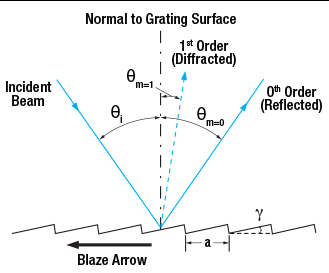
\includegraphics[width=0.4\textwidth]{images/ThorlabsGratingTutorial.png}
\end{figure}

The polar plot of the diffracted light needs to be plotted from 400nm to 1700nm to confirm that no part of the beam travels back in the direction of its source, where it cannot be easily separated. The first, second, and third orders of diffraction off a 1200 g/m grating are shown below, calculated with an incident beam of 45 degrees. Orders two and three are reflected back into the incoming 45 degree beam. Order one is more contained, with whole spectrum falling between 38 and -21 degrees from normal.

\begin{figure}[H]
    \caption{Diffraction angle calculation}
    \centering
    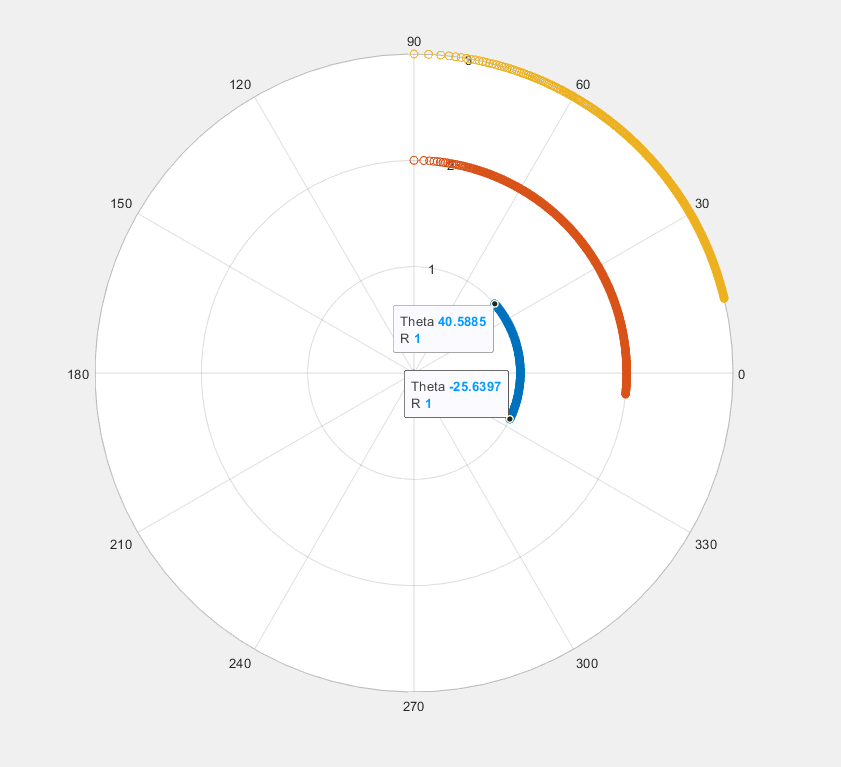
\includegraphics[width=0.75\textwidth]{images/DiffractionAngleCalculator.png}
\end{figure}

The beam coming out of the fiber will have a nonzero width. When the 1.7mm diameter beam hits the surface of the grating, since the grating is at 45 degrees from the beam, light will be propagating from an area with a diameter larger than 1.7mm.

\begin{equation}
    1.7mm/cos(45) = 2.4mm
\end{equation}

This means the spread of the diffracted light will be 38 degrees in and 21 degrees out from both the near edge and the far edge of the collimated beam on the surface of the grating. In order to capture this light and sort it so that the scanner can proceed linearly through each band, we will need a focusing optic that covers the full angular range.

\begin{figure}[H]
    \caption{Basic Ray Trace}
    \centering
    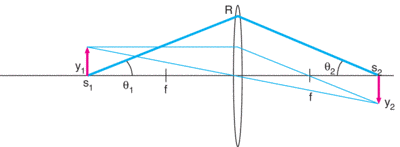
\includegraphics[width=0.75\textwidth]{images/BasicRayTrace.png}
\end{figure}

\paragraph{Focusing Lens} The diffraction grating will diverge the beam away from the sensor surface. This divergence can be corrected with a lens, focusing the divergent light to a spot the size of the sensor or smaller. There are two lens designs that could work, spherical and cylindrical. Spherical lenses are polished with a radius of curvature along both the horizontal and vertical axes. The advantage of a spherical lens is that they are generally cheaper to manufacture and available in a wider variety of sizes and shapes. The spot size of a circular beam passing through a spherical lens will be determined by the distance from the focal length, and the spot will be circular. Cylindrical lenses are cut with a radius of curvature along the horizontal axis, but flat along the vertical axis. A circular beam that passes through a cylindrical lens will be focused to the shape of an ellipse, allowing for more vertical flexibility of alignment. Plano-cylindrical lenses offer another advantage, they have a flat bottom, perpendicular to their planar back. This means they can be stood upright and pressed against a flat surface, dramatically reducing the complexity of the optical mount required to hold them in place. Unfortunately, cylindrical lenses are a specialty part with a smaller market, due to their elliptical focusing pattern, and this turned out to make them cost prohibitive for the project. The dimensions and position of the lens are determined by two things, the angular range of the spatially separated beams coming off the reflective diffraction plate, and the width of the scanning region. 

\begin{figure}[H]
    \caption{Sensor Ray Trace}
    \centering
    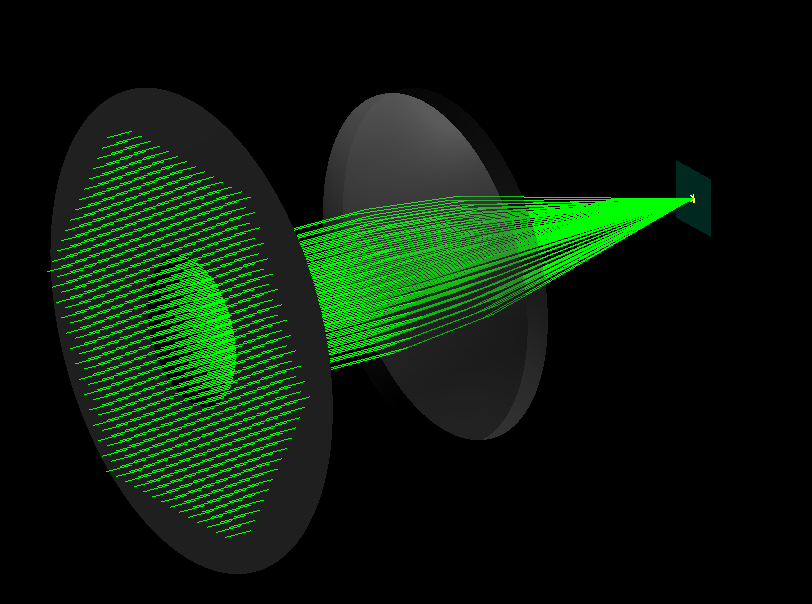
\includegraphics[width=0.5\textwidth]{images/ColimatedBeam.png}
\end{figure}

The lens is also constrained by the angle and width of the input beam, as shown in the ray trace below. If the width of the lens comes within a few wavelengths of the beam approaching the diffraction plate, the beam will diffract around its edge. The size of the detector is 1.36mm across, and the beam needs to be focused from the full angle of about 60 degrees. This means the lens needs an effective focal length of approximately 50mm. In order to prevent the input beam from clipping on the lens, its diameter or height must be at most 30mm, just over 1 inch. 

\begin{figure}[H]
    \caption{Ray Trace of Diffraction Grating}
    \centering
    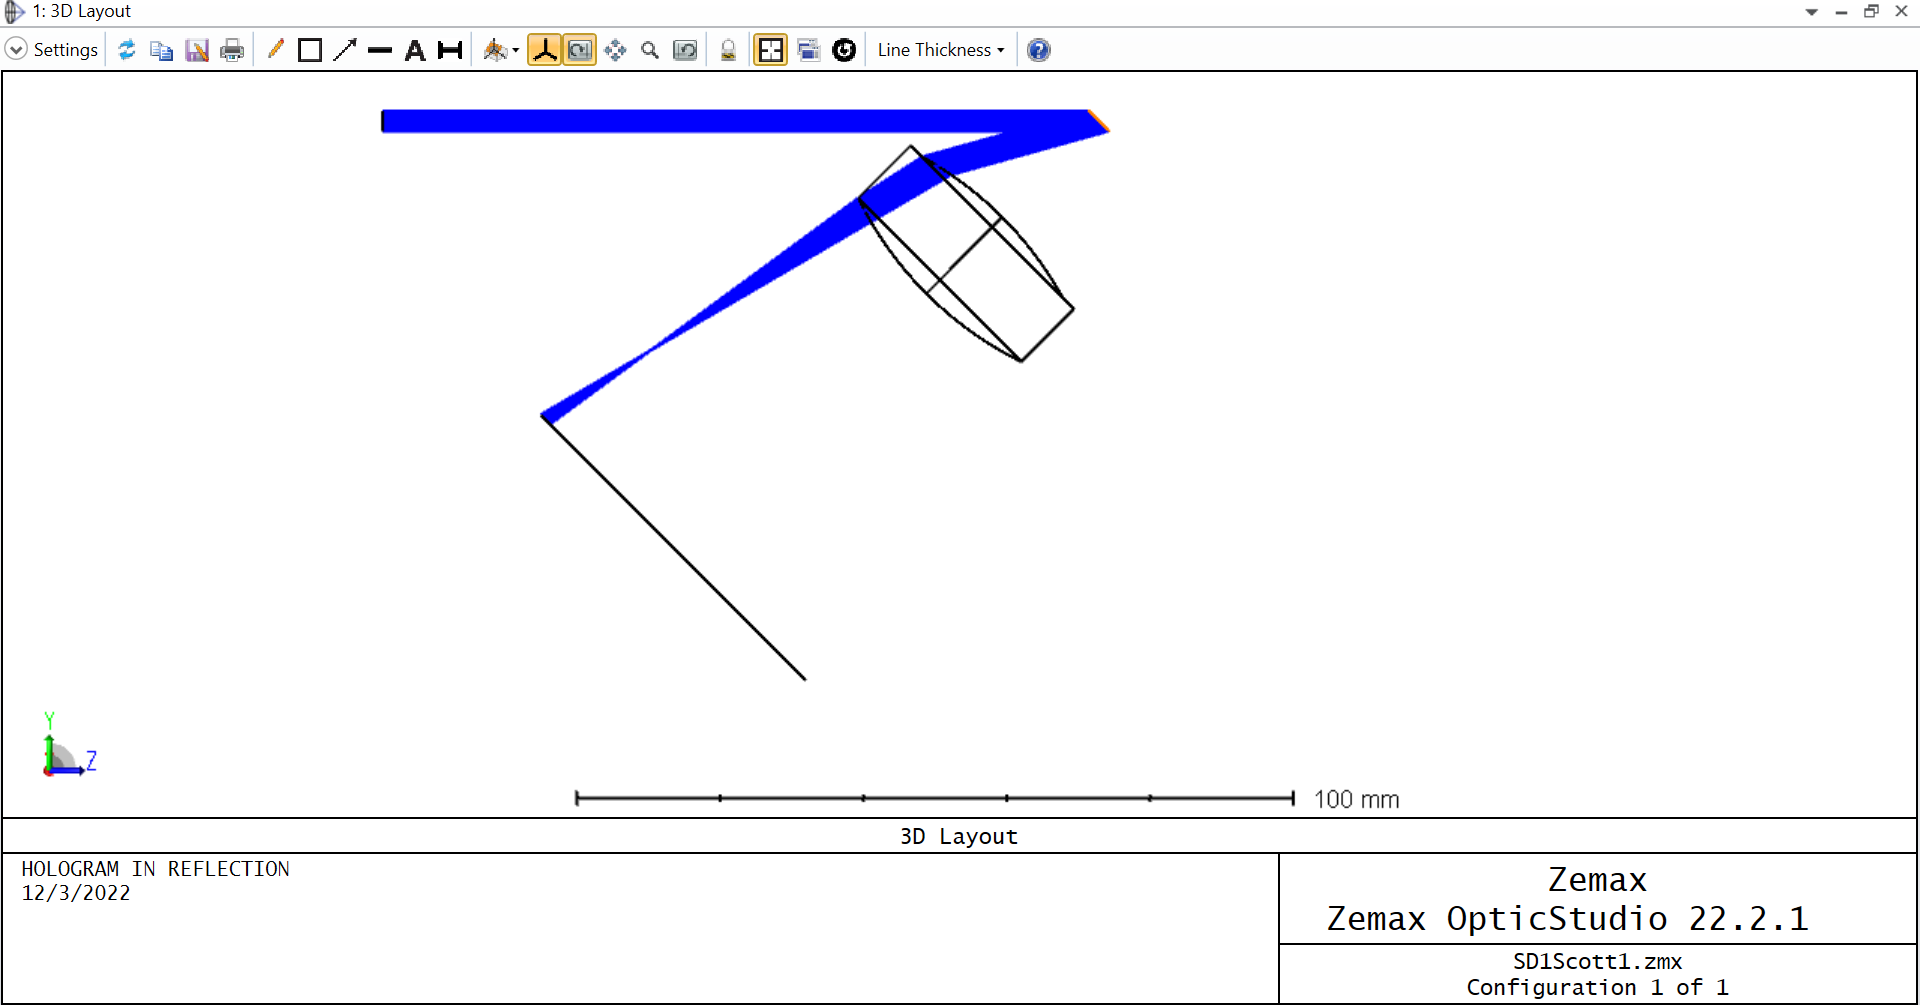
\includegraphics[width=0.75\textwidth]{images/Zemax Ray Trace.png}
\end{figure}

\paragraph{Linear Actuator Rail} The purpose of the linear actuator rail is to carry the sensors to each of the spatially separated beams and hold them in place while the circuit group records the optical power in that position. The size of the sensors can be reduced by covering the button housing with tape so that only a slit is passable, however the minimum distance the linear rail can step is fixed. Stepper motors work by attracting the teeth of a fine magnetic gear in four directions around a pivot point. This translates into torque, which pushes the rail at a rate proportional to the pitch of the turning screw. The equation for step size is:

\begin{equation}
    d = Thread Pitch * (Step Angle / 360 degrees)
\end{equation}

With the minimum step size being 1 pulse. For this motor, the minimum step size is calculated to be 5um, but it is not rated for position accuracy greater than 50um. If the circuit group can record the optical power fast enough, then the rail will not need to stop moving, and position accuracy can be discarded in favor of zero acceleration speed. Otherwise, the 50mm long rail will have room for 1000 precision steps. This should be sufficient for the spectrograph. There are only 1300 discrete wavelengths within the target range, and there is no need to stop at each one. System optimization will involve determining how many wavelengths can be skipped or squeezed together to increase beam precision before having a detrimental effect on the analysis of the spectrograph.

\paragraph{Optical Sensor} The active area of the smaller diode is 1.36 mm squared. Since both sensors will have to pass through the same spatially separated beams with no mechanism for reposition or rearrangement, the beams will have to be focused according to the smaller diode. If the beams were focused on the much more generous 7 mm squared active area of the visible diode, much of the optical power would be lost outside the edges of the near infrared diode.

\begin{figure}[H]
    \caption{Spectrometer Ray illustration}
    \centering
    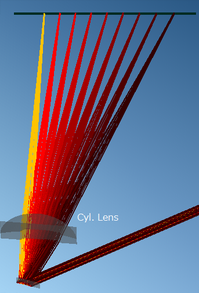
\includegraphics[width=0.25\textwidth]{images/YuanCaoSpectrometer.png}
\end{figure}

\subsubsection{Circuit Group}

\paragraph{Circuitry} The photodiode works by converting a small portion of the incident light into electrical current across the face of the semiconductor. There are three components to the sensing circuitry. First, there is a voltage divider. This voltage divider provides a clean and stable 1.65V to the anode of the photodiode. The photodiode is reversed bias to create a current when detecting light. From there the second part of the circuit begins which is a current-to-voltage converter. The photodiode is emitting a current based on the power of light that is hitting the surface per the area that it is hitting. Using a 100 M$\Omega$ resistor converts current to voltage at a rate of 1 pA to 100 $\mu$V. There are two issues with this however, first the ADC only has 12-bits and as discussed in the controller section, this results in about half a milli-Volt per step. This means that the system is losing about 4x the resolution of the sensor. This is where the last part, the instrumentation amplifier takes effect. The instrumentation amplifier will take the difference between the voltage output and a reference voltage and scale all the parts. For example, if the output voltage of the current-to-voltage converter is .3V (which happens to be the dark current of the visible light sensor) subtract the voltage of the dark current and scale. This current will be detected as voltage by the microcontroller, which will then record the signal strength and assign it a wavelength. The resulting data set is a spectrograph the remainder will help.
\begin{figure}[H]
    \caption{Sensing Schematic}
    \centering
    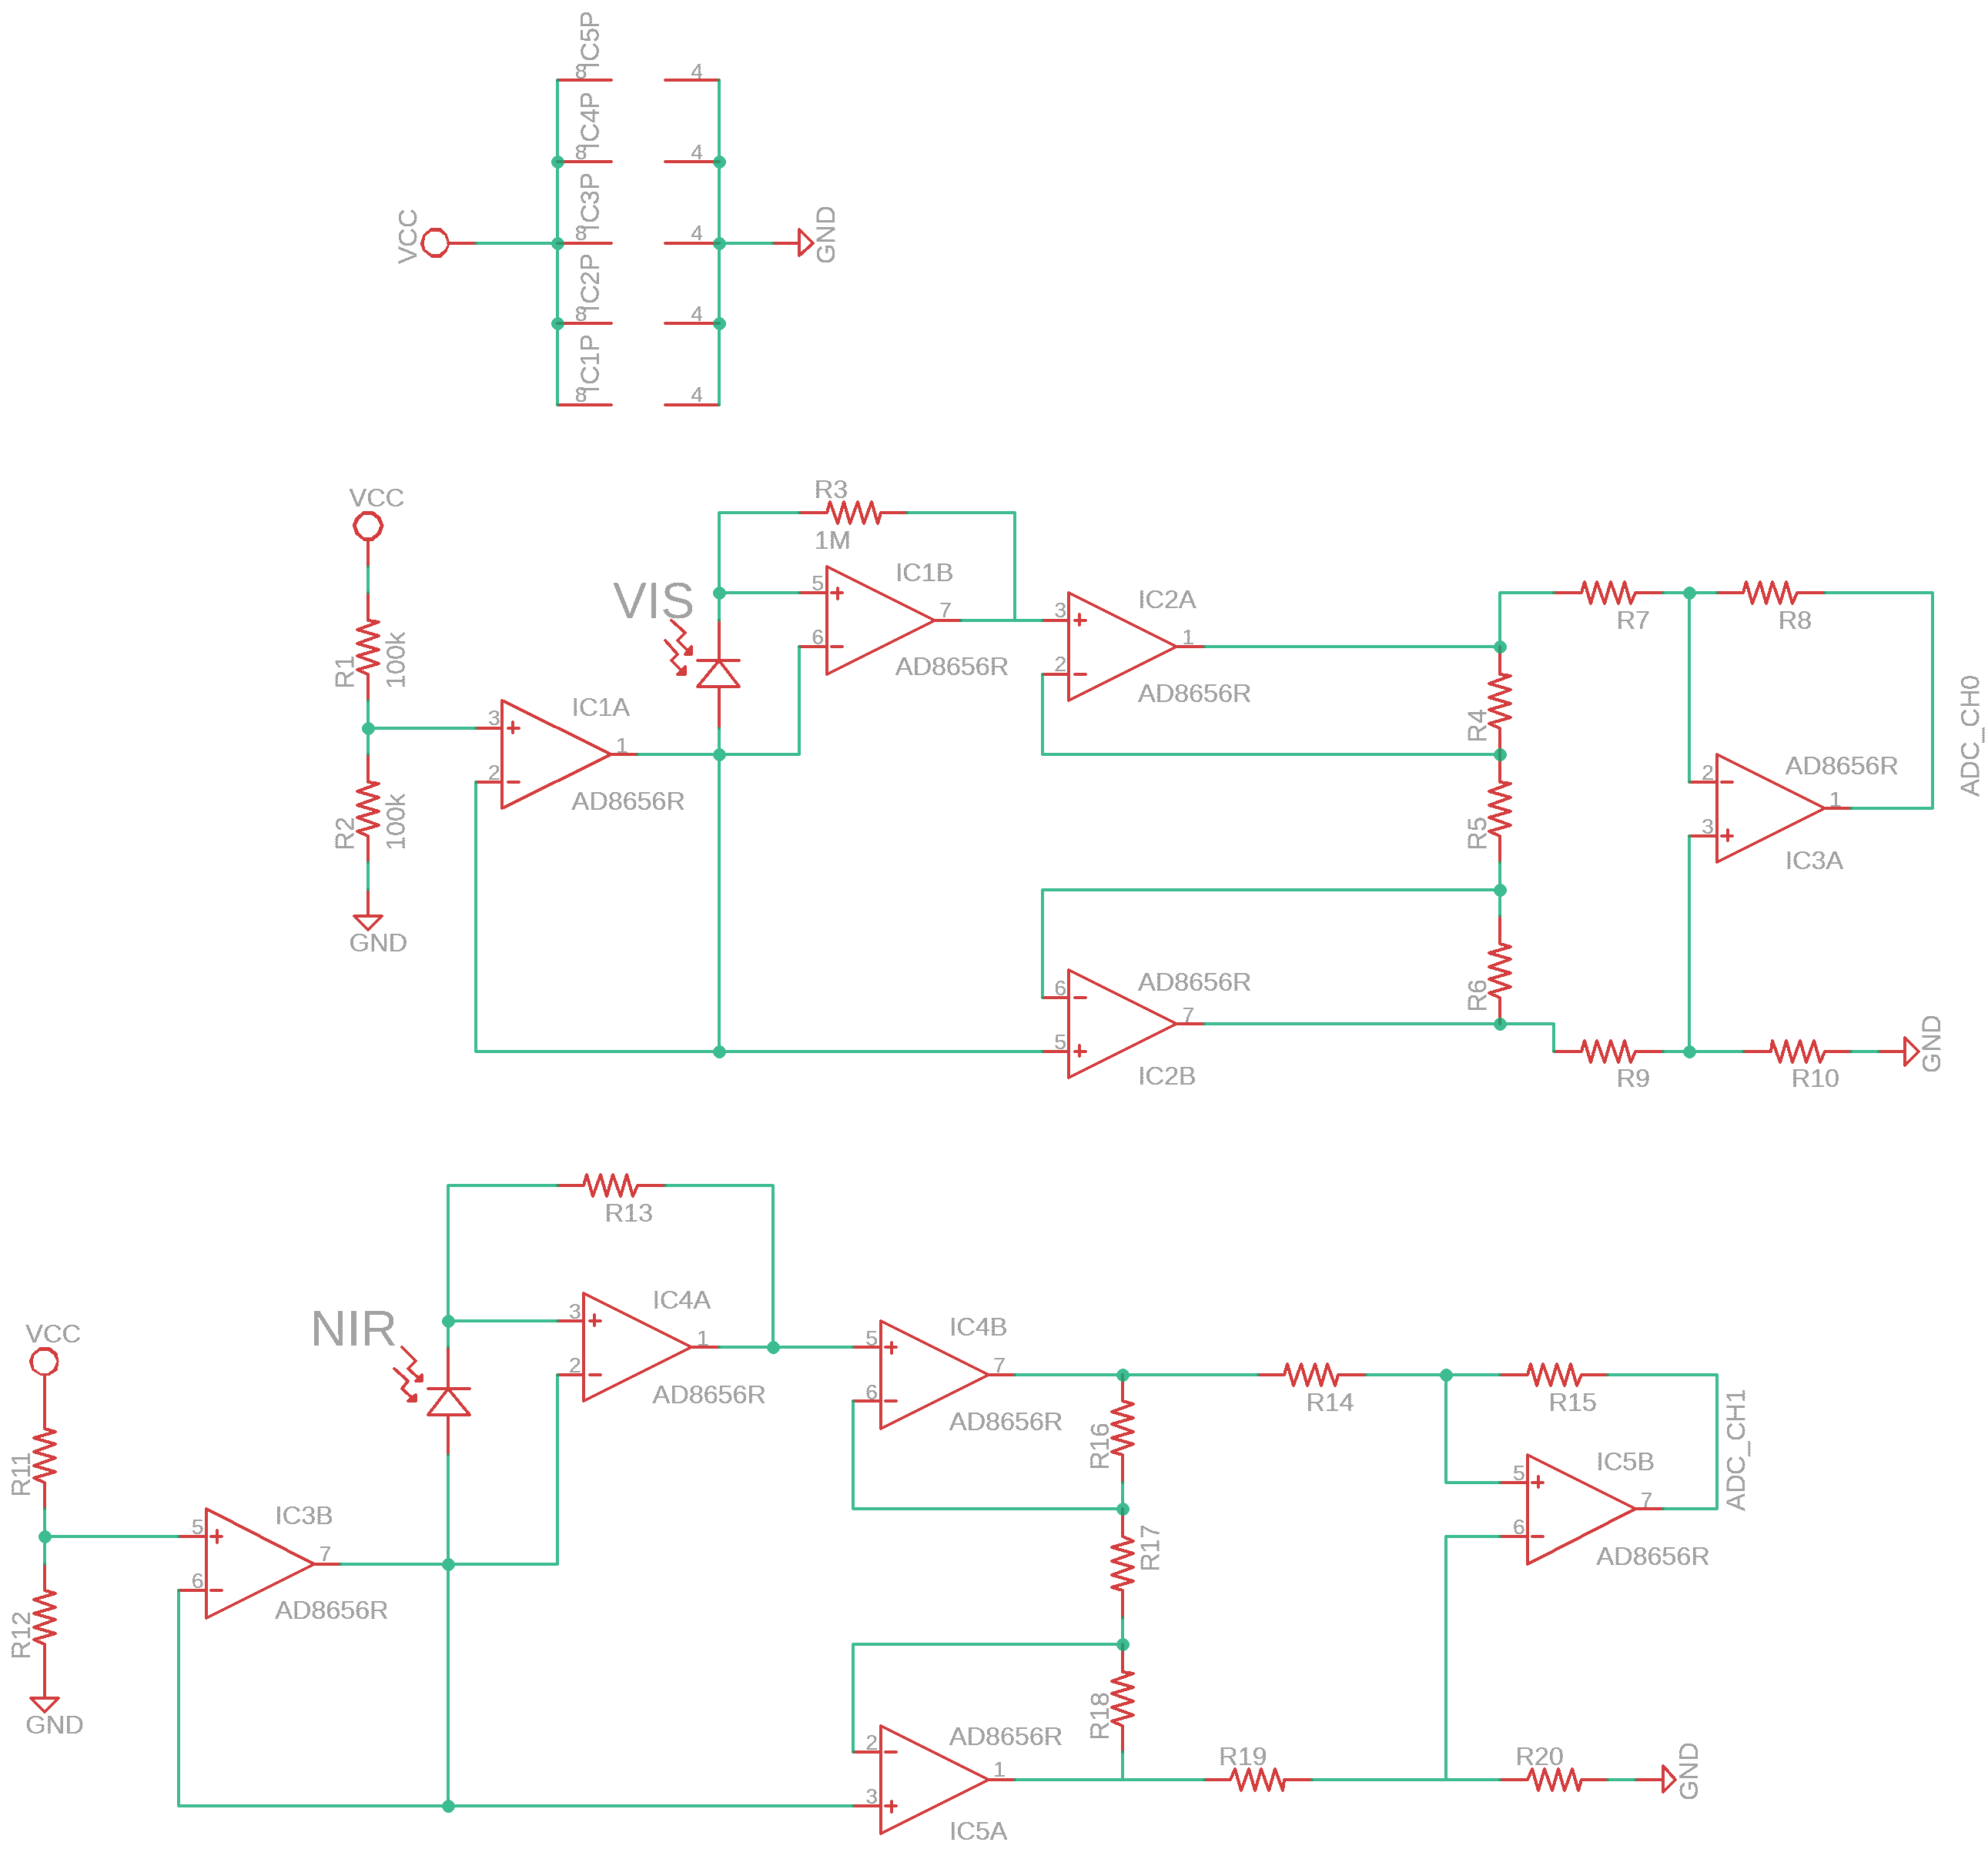
\includegraphics[width=.8\textwidth]{images/sensor-schematic.png}
    \label{fig:sensor-schem}
\end{figure}

\paragraph{Spectrograph} The spectrograph created by the microcontroller will have the information contained in the soil. However, this information will need to be extracted from the spectrograph in different ways for different data. Two problems must be overcome, signal strength and calibration. The reflectance amplitude can be optimized by making adjustments to the circuitry and the optical alignment. Calibration requires a large dataset of soil from the same source as our garden bed. If this cannot be obtained from university botanical resources or open source libraries, it can be done by selecting samples and borrowing a spectrometer.

\begin{figure}[H]
    \caption{Soil Spectrograph}
    \centering
    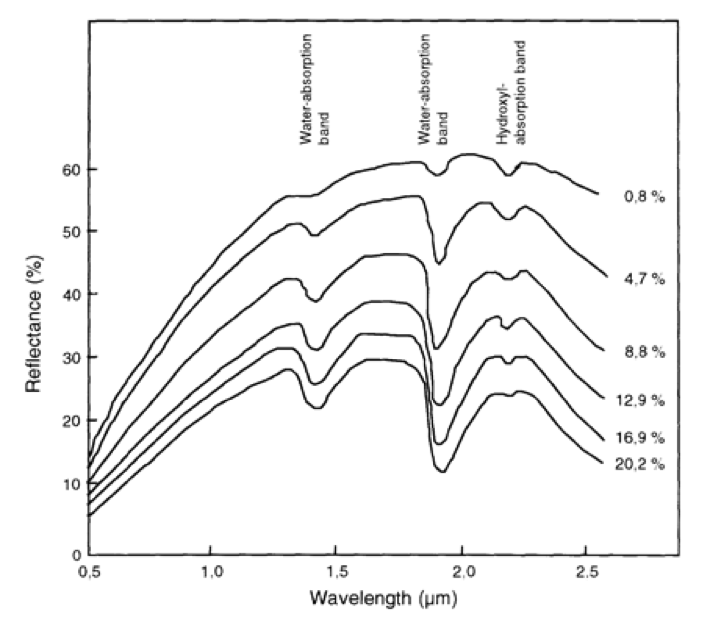
\includegraphics[width=0.75\textwidth]{images/GenericSoilSpectra.png}
\end{figure}

